\documentclass[a4paper,12pt,bibliography=totoc]{article}
\usepackage[utf8]{inputenc}
\usepackage{graphicx}
\usepackage[hidelinks]{hyperref}
\usepackage{array}
\usepackage{lastpage}
\usepackage{lipsum}
\usepackage{wrapfig}
\usepackage{multirow}
\usepackage{url}
\usepackage{fancyhdr}
\usepackage{titling}
\usepackage{lastpage}
\usepackage[page]{totalcount}
\usepackage[table]{xcolor}
\usepackage{authblk}
\usepackage{csquotes}
\usepackage{epigraph}
\usepackage{movie15}
\usepackage{subcaption}
\usepackage{soul}
\usepackage{pbox}
\usepackage{xcolor}
\usepackage[hmargin=2cm,top=5cm,headheight=75pt,footskip=25pt]{geometry}

\setlength{\parindent}{0.95cm}

\setlength{\epigraphwidth}{0.9\textwidth}


\pagestyle{fancy}

\fancyhf{}
\renewcommand{\headrulewidth}{0pt}
\fancyhead[C]{%
          \setlength{\extrarowheight}{8pt}
          \renewcommand{\arraystretch}{1}
          \begin{tabular}{|m{3.0cm}|m{4.0cm}|m{3.0cm}|m{4.8cm}|}
          \hline
          % start row 1  
		  \multirow{3}{*}{
          	
\includegraphics[width=2.5cm]{logo-dsoft.png}
          } & \multicolumn{3}{m{11.8cm}|}{ 
          	\raggedleft \color[rgb]{.6, 0, 0} \large \fontfamily{ugq}\selectfont DSOFT - Vietnam Joint Stock Company
          } \tabularnewline
          %& 
          %\centering
          %\Huge{TITLE} &
          %\centering
          %\tiny{P\'ag. \thepage\ de \pageref{LastPage}\\
          %Data: 17/05/2013\\
          %Rev. 0}
          \cline{2-4}    
          % start row 2    
          \renewcommand{\arraystretch}{1}     
           & \multicolumn{2}{m{7.0cm}|}{\raggedleft \footnotesize Capstone Project 1 }
          & \raggedleft \scriptsize \url{http://www.d-soft.com.vn}         
          \tabularnewline
          \cline{2-4}    
          % start row 3         
           & \raggedleft \footnotesize Reference: 
           & \raggedleft \footnotesize Revision: 0.1 
           & \raggedleft \scriptsize \url{dsoft@d-soft.com.vn}                  
          \tabularnewline
          \hline        
          \end{tabular}%
}
\renewcommand{\footrulewidth}{0.4pt}
\rfoot{\small Page: {\thepage} of {\getpagerefnumber{LastPage}}}
\lfoot{\small D-Soft ML Training Course}


\fancypagestyle{plain}{%
\renewcommand{\headrulewidth}{0pt}
\fancyhead[C]{%
          \setlength{\extrarowheight}{8pt}
          \renewcommand{\arraystretch}{1}
          \begin{tabular}{|m{3.0cm}|m{4.0cm}|m{3.0cm}|m{4.8cm}|}
          \hline
          % start row 1  
		  \multirow{3}{*}{
          	
\includegraphics[width=2.5cm]{logo-dsoft.png}
          } & \multicolumn{3}{m{11.8cm}|}{ 
          	\raggedleft \color[rgb]{.6, 0, 0} \large \fontfamily{ugq}\selectfont DSOFT - Vietnam Joint Stock Company
          } \tabularnewline
          %& 
          %\centering
          %\Huge{TITLE} &
          %\centering
          %\tiny{P\'ag. \thepage\ de \pageref{LastPage}\\
          %Data: 17/05/2013\\
          %Rev. 0}
          \cline{2-4}    
          % start row 2    
          \renewcommand{\arraystretch}{1}     
           & \multicolumn{2}{m{7.0cm}|}{\raggedleft \footnotesize Capstone Project 1 }
          & \raggedleft \scriptsize \url{http://www.d-soft.com.vn}         
          \tabularnewline
          \cline{2-4}    
          % start row 3         
           & \raggedleft \footnotesize Reference: 
           & \raggedleft \footnotesize Revision: 0.1 
           & \raggedleft \scriptsize \url{dsoft@d-soft.com.vn}                  
          \tabularnewline
          \hline        
          \end{tabular}%
}
}

\setlength\parindent{12pt}



\title{
%
\includegraphics[width=18cm]{img/logo-dsoft.png} \\
%\vspace*{6cm}
\textbf{Age and Gender Classification} \\
\textit{(Specifications)}
}

\author{
Bui Gia Huy\thanks{Artificial Intelligence Department} \thanks{Email: \url{huygb@vietnews24.com}}
}
\date{\textbf{\today}}


%\fancyfoot[C]{%
%          \begin{tabular}{|m{3.0cm}|m{10.0cm}|m{2.5cm}|}
%          \hline
%          \includegraphics[height=1.5cm,width=2.5cm]{logo.png} &
%          \centering
%          \Huge{TITLE} &
%          \centering
%          \tiny{P\'ag. \thepage\ de \pageref{LastPage}\\
%          Data: 17/05/2013\\
%          Rev. 0}\tabularnewline
%          \hline
%          \end{tabular}%
%}
\usepackage{graphicx}
\graphicspath{ {./figs/} }
\begin{document}
%--------------------Title Page
\maketitle
\newpage
%--------------------Change Log Page
\begin{center}
\setlength{\extrarowheight}{5pt}
\begin{tabular}{|m{1cm}|m{4cm}|m{2.5cm}|m{2cm}|m{2.5cm}|m{2cm}|} 
 \hline
 \multicolumn{6}{|m{17cm}|}{\cellcolor{red!25} \Large \textbf{DOCUMENT CHANGE LOG}}
 \\
 \hline
\centering \textbf{Rev.} & \centering \textbf{Description} & \centering \textbf{Author} & \centering \textbf{Date} & \centering \textbf{Approved} & \textbf{Date} \\
 \hline
 0.1 & Draft 1 & Huy G.B & 2019/03/04
 & & \\
 \hline
 &  &  &  & & \\
 \hline
 &  &  &  & & \\
 \hline
 \multicolumn{6}{|m{17cm}|}{\cellcolor{red!25} This document has been based on template TL-SSW-101 Revision 2.0}
 \\
 \hline
\end{tabular}
\end{center}
\newpage
%--------------------ToC Page
\tableofcontents
\newpage
%--------------------Begin Outline
\section{Introduction}
- This \textit{Casptone Project 1} assits for my learning about Machine learning and Deep learning in training course of D-Soft company that Mr. Trung Anh is my supervisor. \\
- Through this project, i want to improve some skills about coding, researching relate to machine learning.\\
- It has a lot of interesting applications about machine learning but in this project i will choose topic \textbf{Age and Gender Classification} because D-Soft company where i am working, has a project relate to this problem.

\subsection{Purpose}
- Reinforce knownledge about machine learning learned from Coursera \textit{Andrew Ng.}
- Build a funny application that apply machine learning to the real world.
\subsection{Scope}
- This project in range of D-Soft's training course.\\
- The project focus mainly about: \\
\indent + Build a simple web frontend and backend. \\
\indent + Training a machine learning algorithm.

\subsection{Definitions, Acronyms, and Abbreviations} 
\begin{center}
\begin{tabular}{|m{3cm}|m{8cm}|} 
 \hline
 AI & Artificial Intelligence \\
 \hline
 FNN & Feedforward Neural Network \\
 \hline
  & \\
 \hline
  & \\
 \hline
\end{tabular}
\end{center}

\bibliographystyle{unsrt}
\bibliography{references}
1. \url{https://talhassner.github.io/home/publication/2015_CVPR} \\
2. \url{https://talhassner.github.io/home/projects/cnn_agegender/CVPR2015_CNN_AgeGenderEstimation.pdf} \\
3. \url{https://gilscvblog.com/2015/11/19/age-and-gender-classification-using-deep-convolutional-neural-networks/} \\
4. \url{http://dlib.net/} \\
5. \url{https://js.tensorflow.org/} \\
\newpage

\section{Related Works}

- In this section,  I will introduce briefly about my overall system for Capstone Project 1.\\
- Project name: \textbf{Age and Gender Classficication.}\\
\indent + Input: Image\\
\indent + Output: Age, Gender information\\
\indent + Platform: Web App

\begin{center}
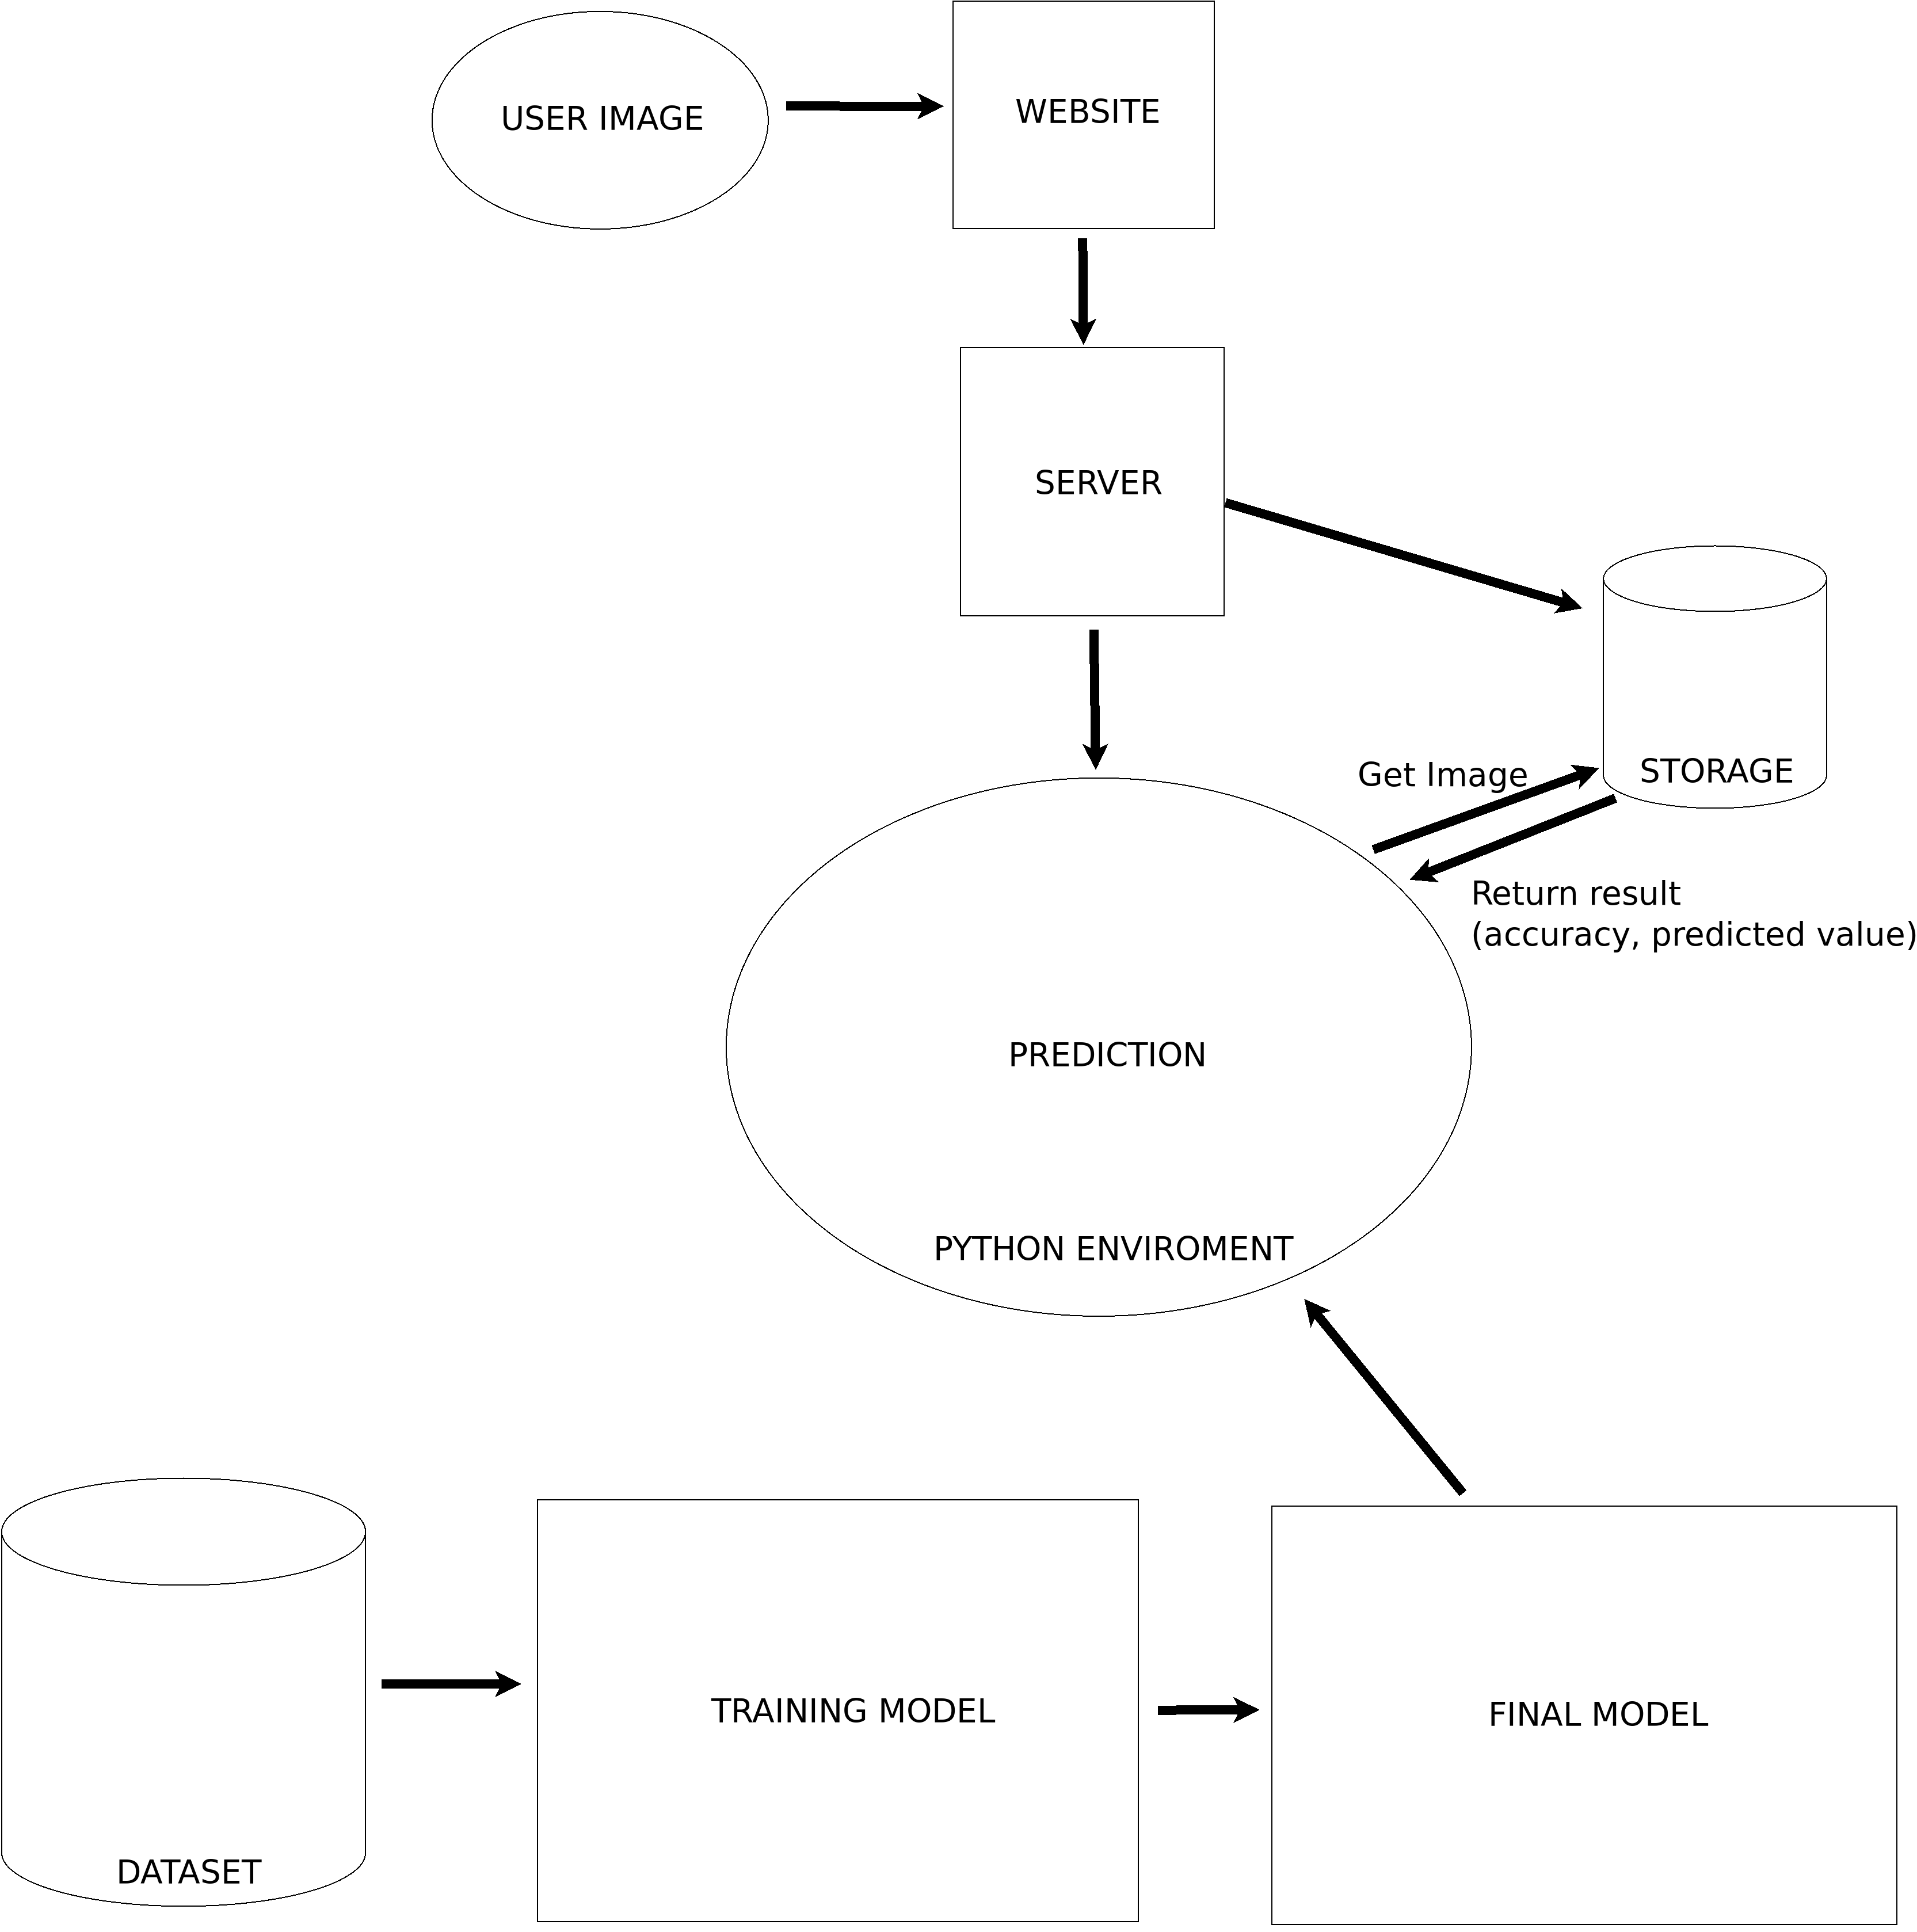
\includegraphics[scale=0.12]{overview} \\
\textit{Figure 1: Overall System (A High level Diagram)}
\end{center}


\newpage
\subsection{Neural Network}
\subsection{Python}
\subsection{Classification}
\subsection{Example: Dog and Cat Classfication}

%%\begin{figure}
%%\centering
%%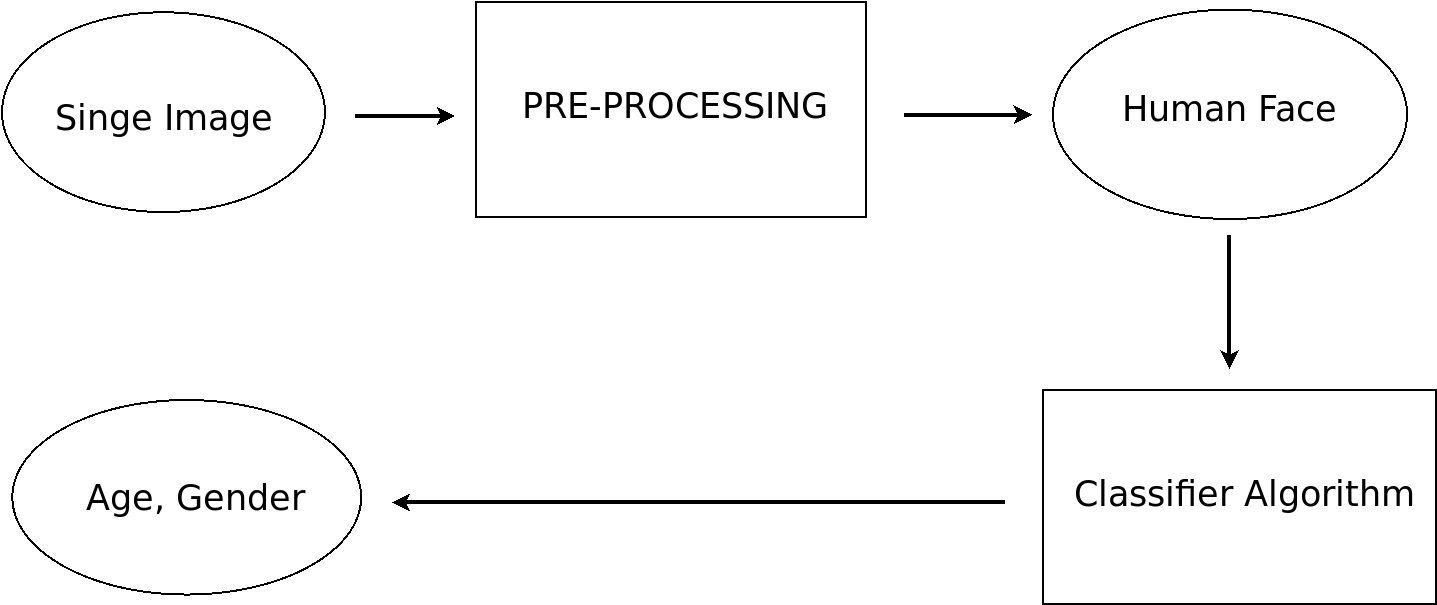
\includegraphics[scale=0.25]{nn_diagram}
%%\end{figure}
\begin{center}
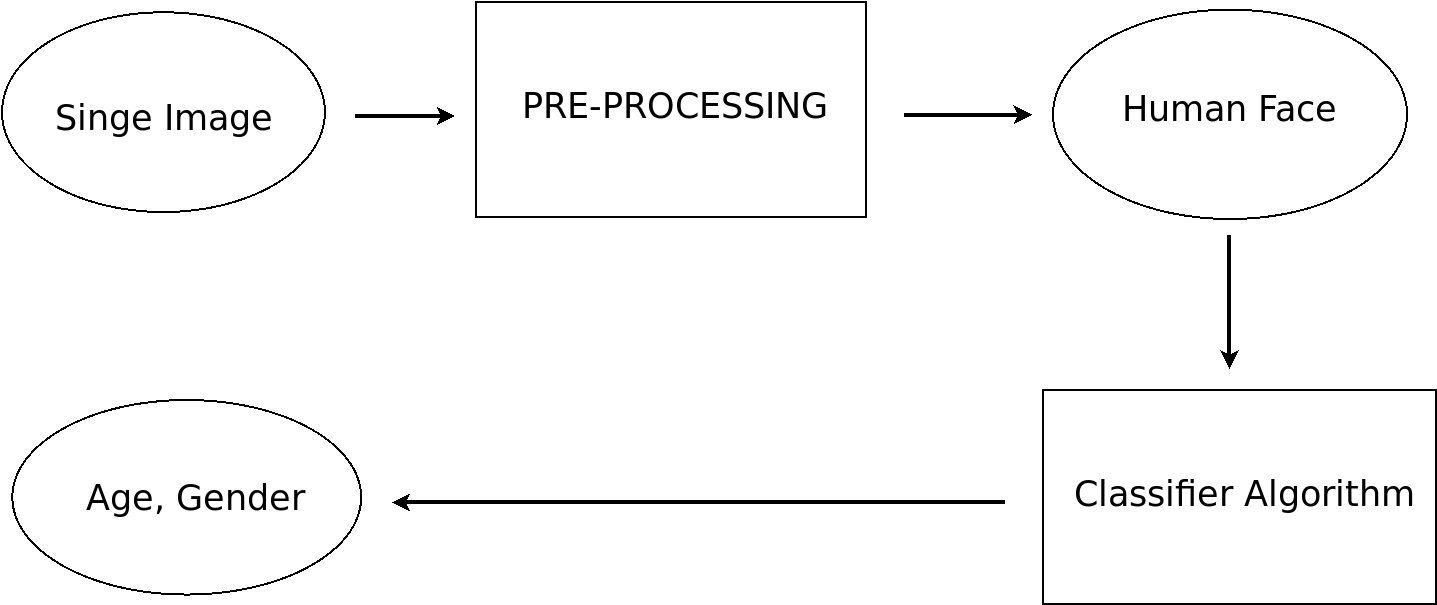
\includegraphics[scale=0.25]{nn_diagram} \\
\textit{Figure 2: Classfication Pipeline}
\end{center}

\subsubsection{Dataset}
- Preparing training dataset for classifier algorithm
- Datasets that i am going to plan to use for my classifier algorithm as follows: \\
 + IMDB-WIKI (\url{https://data.vision.ee.ethz.ch/cvl/rrothe/imdb-wiki/}) \\
 + VISAGE (\url{https://www.forensicsandsecurity.com/visage.php}) \\
 + UTKFace (\url{https://susanqq.github.io/UTKFace/}) \\
 + Blog Posts Labeled with Age and Gender (\url{https://www.kaggle.com/tomlisankie/blog-posts-labeled-with-age-and-gender}
\subsubsection{Pre-processing}
- Grey + crop images in dataset.
\subsubsection{Neural Network as Classifier Algorithm}
- There are a lot of classifier algorithms that we can use. But here, we will use \textbf{Neural Network (NN)} for our problem.\\
- Feedforward Neural Network \textit{(FNN)} is NN architecture that we apply for age and gender classification. Below is basic architecture of it \textbf{(figure 3)}.\\
\begin{center}
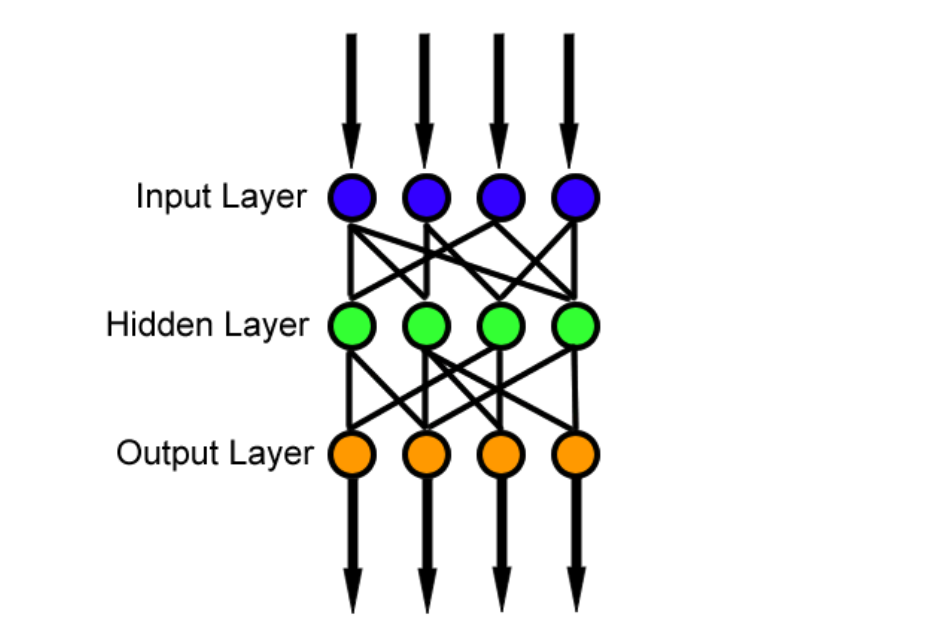
\includegraphics[scale=0.30]{feedforward_architecture} \\
\textit{Figure 3: Feedforward Neural Network}
\end{center}
- In this Capstone Project 1, we just only use FNN. The archictecture is not usually fit for \textbf{computer vision} because it has to have a very high parameters \textit{(weights)} capicity in their model. These problems in computer vision field is often solved efficiently with Convolutional Neural Network \textit{(CNNs)} because it can decrease dramatically large amount of weights in their model but accuracy of model is very high meanwhile still remaining \textit{spatial arrangement} in addtional to \textit{local connectivity}.\\
- Return our problem, our FNN architecture is namely as \textbf{figure 4}. That is a 2-layer neural network, the network's input is image. In training phase, we will use images from \textit{training set} and in test phase, we use ones from \textit{test set}.
Maybe in hyperparameter-tuning phase, we can use \textit{validation set} for regularization.
\begin{center}
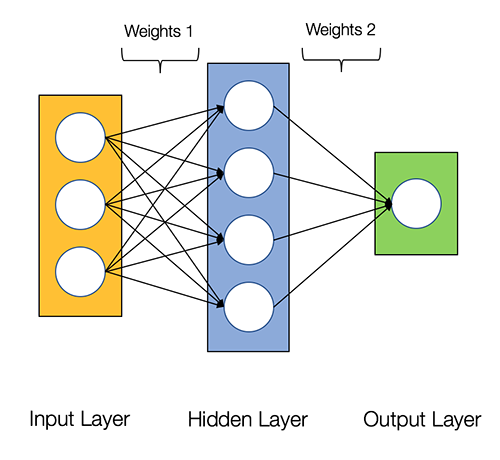
\includegraphics[scale=0.40]{our_network} \\
\textit{Figure 4: 2-layer Neural Network}
\end{center}

\subsection{Web Application}
\subsubsection{Client}
- Clients are some members in our teams :)\\
- User can access to our website for testing purpose.
\subsubsection{Server}
- \textit{Server language}: \textbf{Nodejs} \\
- \textit{Server Framework}: \textbf{ExpressJS} \\

\begin{center}

\includegraphics[scale=0.25]{nodejs-express}
\end{center}

- RESTful APIs with Nodejs and Expressjs Diagram \textit{(non-blocking IO)}:
\begin{center}
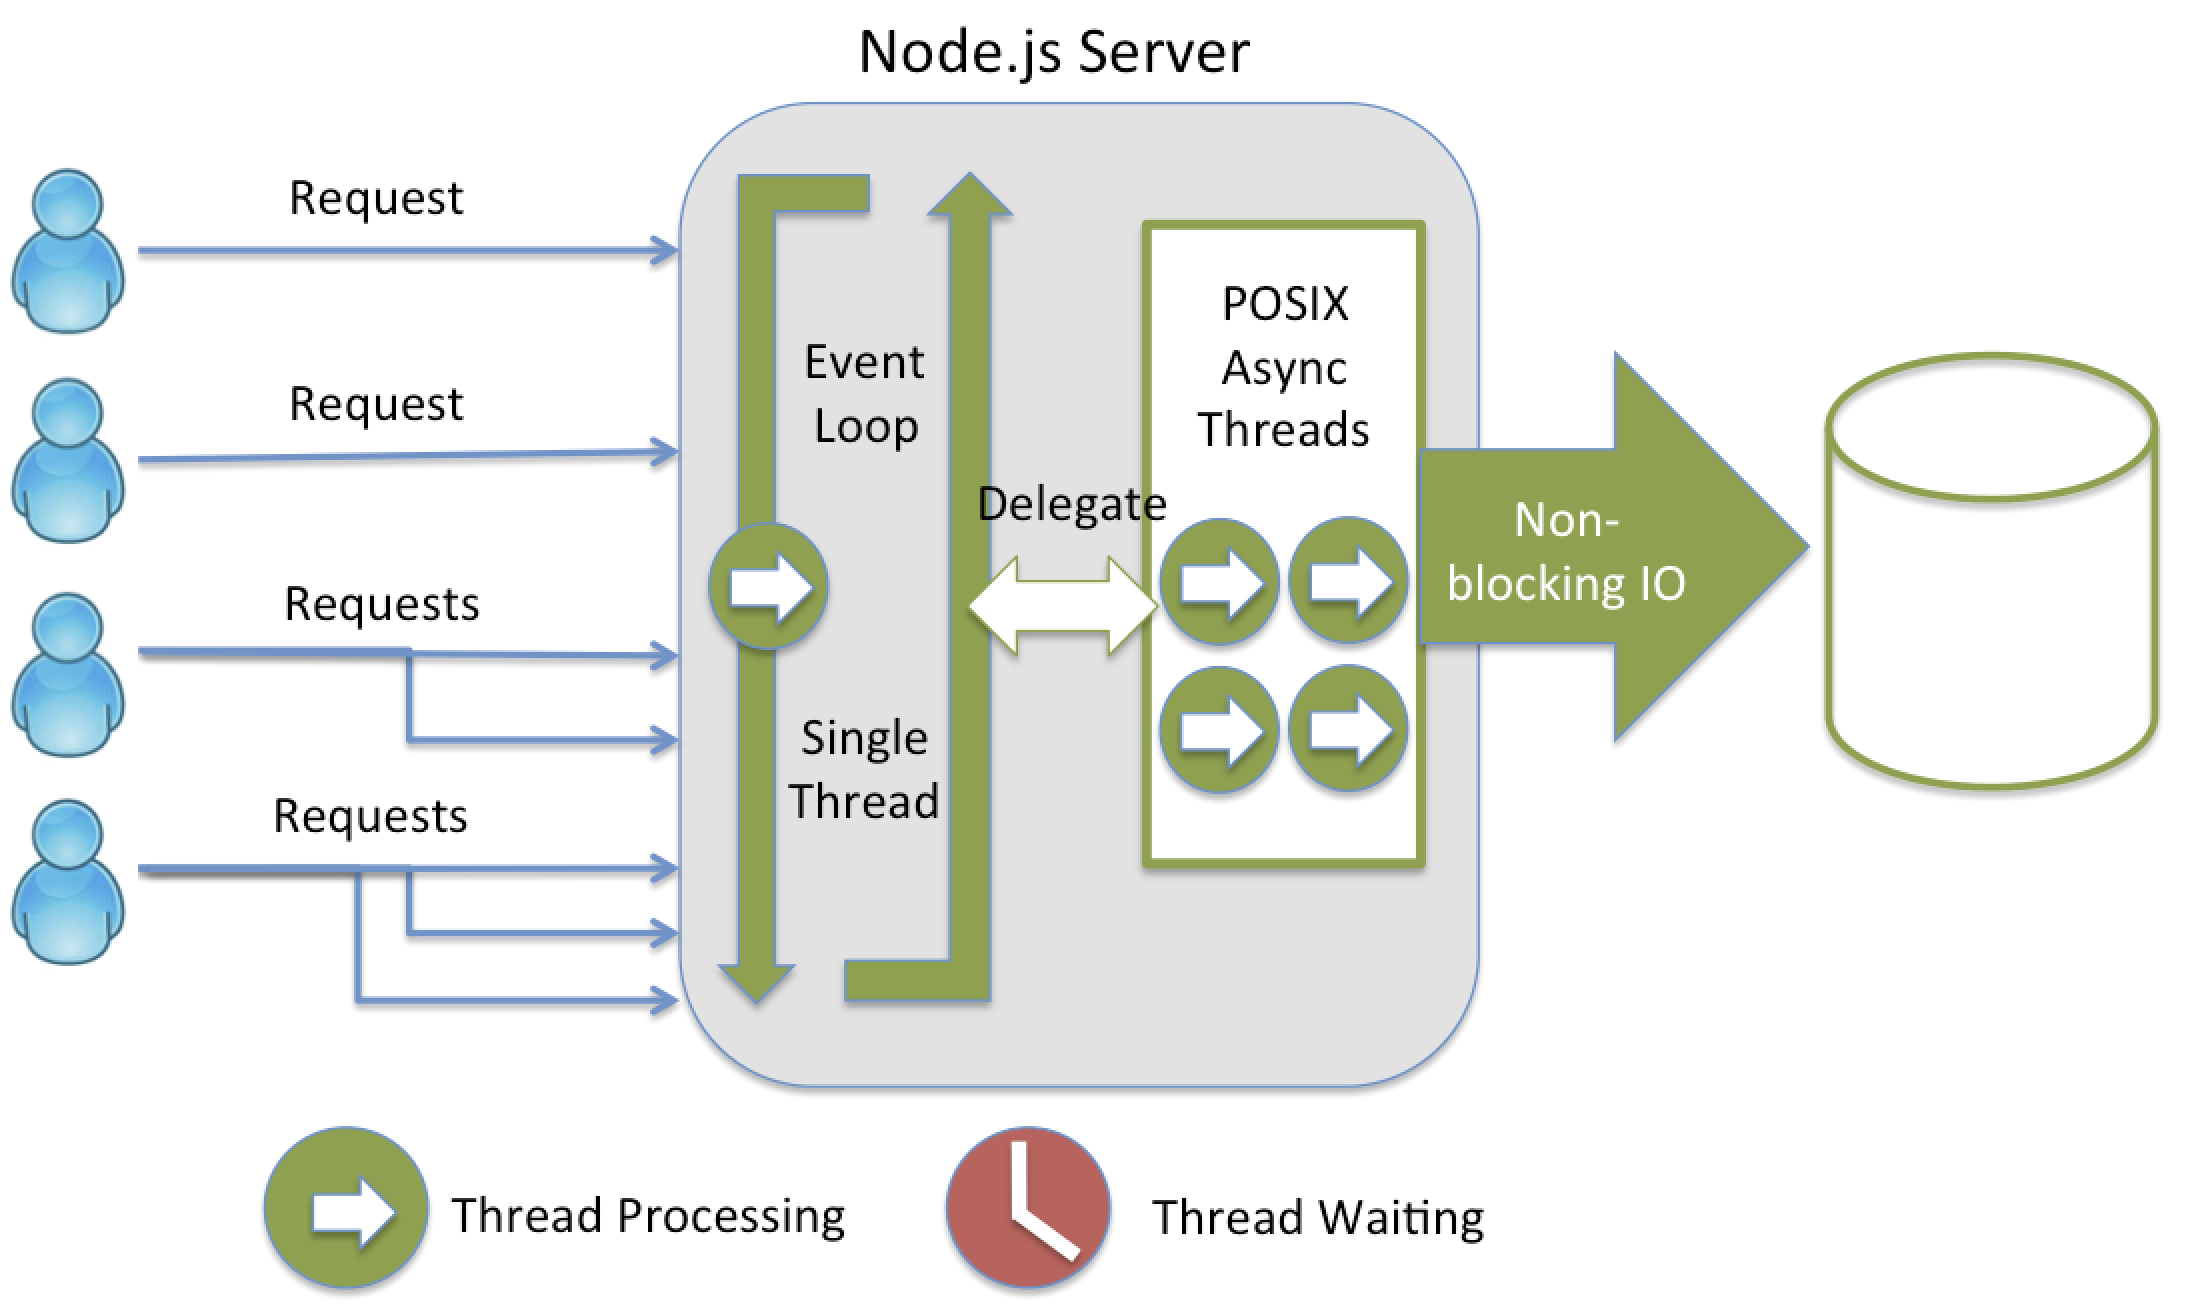
\includegraphics[scale=0.30]{restful-api} \\
\textit{Figure 5: Internal Process of Nodejs}
\end{center}

- My server will reiceives requests from users and holds their images taken from user my local storage. When user submits an image in a given form, it will be sent to my local server through RESTful API. Then, Nodejs server will send it to my Python script for predict Age and Gender with above 2-layer Neural Network depicted such as above.

\newpage
- This figure below is high-level diagram for my backend architecture:\\
\begin{center}
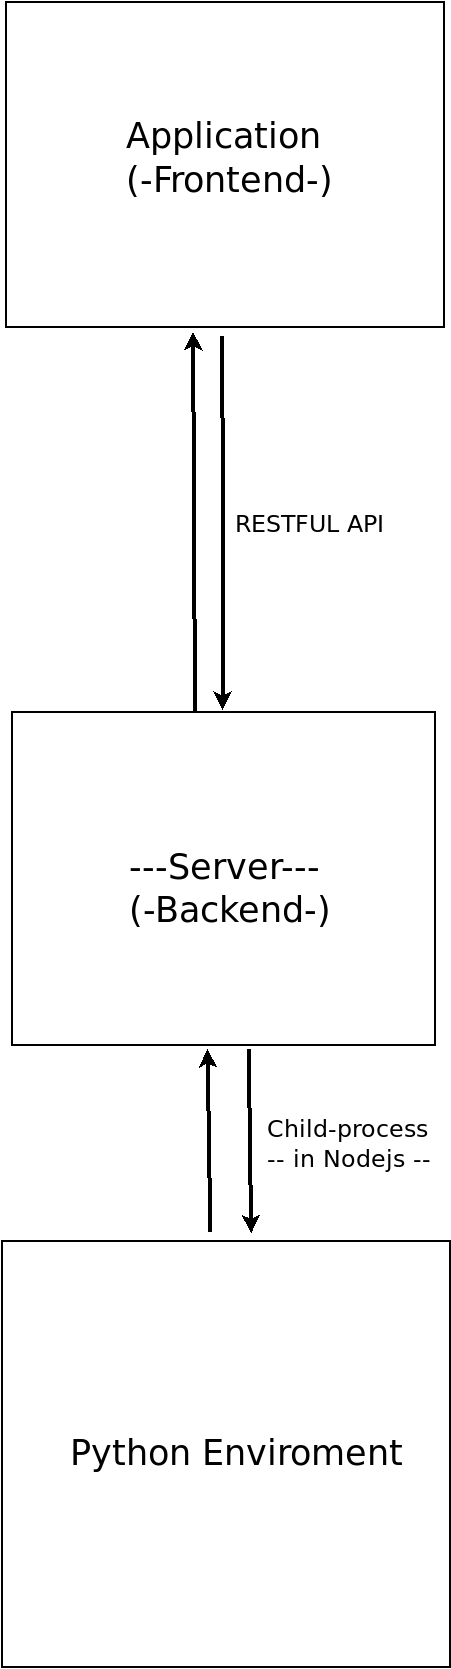
\includegraphics[scale=0.30]{backend} \\
\textit{Figure 6: Backend Architecture}
\end{center}

\newpage
\section{Proposal}
\subsection{Fronted}
\subsection{Backend}
\subsection{Machine Learning}

....

\begin{table}[h]
\begin{tabular}{|m{0.3cm}|m{1.0cm}|m{9.7cm}|m{1.6cm}|m{2.4cm}|}
\hline
\multicolumn{5}{|m{17cm}|}{\cellcolor{red!25} \large\textbf{Work Breakdown Structure \& Estimate}} 
\\
\hline
\textbf{\#} & \multicolumn{3}{|m{12.3cm}|}{\textbf{Activities}} & \pbox{2.4cm}{\textbf{~Expected} \\ \textbf{(man-days)}}
\\
\hline
\textbf{1} & \multicolumn{2}{|m{10.7cm}|}{\textbf{Preparation}} & \textbf{1} & 
\\
\hline
& 1.1 & Setup the development environment & & 0.5
\\
\hline
& 1.2 & Search + Pre-processing Dataset & & 0.5
\\
\hline
\textbf{2} & \multicolumn{2}{|m{10.7cm}|}{\textbf{Design and Implement}} & \textbf{3} &
\\
\hline 
& 2.1 & Training + Testing model & & 2
\\
\hline
& 2.2 & Frontend + Backend & & 1
\\
\hline
\multicolumn{2}{|m{1.3cm}|}{} & \multicolumn{2}{m{11.3cm}|}{} &
\\
\hline
\multicolumn{2}{|m{1.3cm}|}{} & \multicolumn{2}{m{11.3cm}|}{\hl{\textbf{Total (man-days)}}} & \hl{\textbf{4}}
\\
\hline

\end{tabular}%
\end{table}

\end{document}